
DNA is the general medium of information common to all known living creatures. It defines all the traits that all the individuals from a species share, and thus, is the most important source of biological information for species definition and the understanding of life in general. This code is replicated when a cell goes under mitosis, ensuring that the whole organism has a coherent DNA code across all its cells.

DNA takes the form of a long string of proteins, linked two by two. These proteins are called "nucleotides" or "bases", as they are the base of the DNA code. There are four of them: adenine [A], thymine [T], cytosine [C] and guanine [G], often referred to by their initial for ease of use. Adenine and thymine are linked together, and cytosine and guanine are also paired together, forming a double-helix, as shown on Figure~\ref{fig:double-stranded-dnamed}.

\begin{figure}[h]
	\centering
	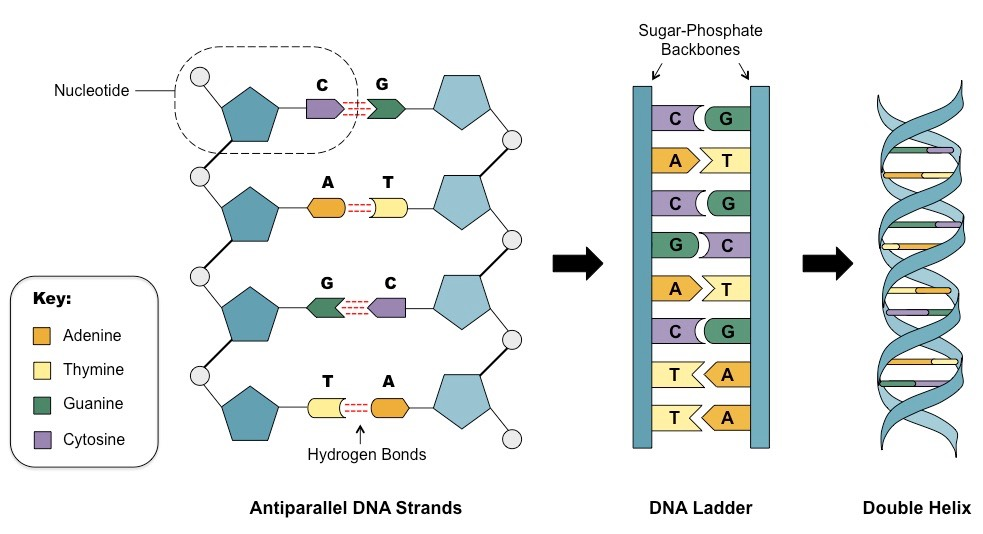
\includegraphics[width=1\linewidth]{double-stranded-dna_med}
	\caption{DNA double-helix with nucleotides (from~\cite{cornell:dnastructure})}
	\label{fig:double-stranded-dnamed}
\end{figure}


An important factor of differentiation in the characteristics in different species is mutation, when a random modification appears in the DNA code and propagates across the population with reproduction. If the mutation gives the bearer an advantage in life over the non-bearers, it has a high probability to get passed to the bearer's descendants, fostering its propagation in the population (for example, having coloured petals for flowers makes them attractive for insects, and since coloured flowers have become more pollinated, their heirs will inherit this trait). On the contrary, if the mutation becomes a drawback, it is unlikely to be passed to the descendants.

Some genetic mutations are proven deadly, and the most well-known in this category is cancer. A cell whose DNA has been damaged or altered can start multiplying in an uncontrollable fashion, creating a pack of cells growing ever bigger, becoming malign and threatening the normal behaviour of an organ. This process, known as carcinoma, can be detected by multiple ways, some more empirical than others (for example, an easy setup with X-rays can allow a doctor to detect a small abnormal spot, which could be a sign of carcinoma). One way to detect this is by getting a sample of DNA from a patient, and comparing it with a known reference.

To achieve this comparison, one needs to find which area of the reference genome matches with the samples, or said differently, one needs to align the sample DNA with the reference and find how similar these two are. Consequently, we define a metric to quantify that closeness, called the \emph{alignment score}.

In this case, only a pair of sequences are being matched: a sample, and a reference. This is called \emph{pairwise alignment}. Other cases where DNA alignment is needed can involve comparing multiple species' DNA to find regions that share some similarity, and that could translate into shared trait among species. In that situation, multiple sequences are mapped together, which makes it yet another problem.